    \problem
    \begin{question}
        Check if the following equation is exact
        \[dX_t=(2tW_t^3+3t^2(1+W_t))dt+(3t^2W_t^2+1)dW_t, X_0=0.\]
        Then find the solution of this SDE.
    \end{question}
    Denote the drift pattern $a(t,W_t)=2tx^3+3t^2(1+x)$
    and the volatility pattern $b(t,x)=3t^2x^2+1$, then
    it easy to see that
    \[\frac{\partial a}{\partial x}
    =\frac{\partial b}{\partial t}+
    \frac{1}{2}\frac{\partial^2 b}{\partial x^2}
    =6tx^2+3t^2\]
    It follows that this is an exact equation, hence the
    corresponded function $f(t,x)$ satisfies
    \[\left\{\begin{aligned}
        &\frac{\partial f}{\partial t}+\frac{1}{2}\frac{\partial^2 f}{\partial x^2}
        =2tx^3+3t^2(1+x)\\
        &\frac{\partial f}{\partial x}=3t^2x^2+1
    \end{aligned}\right.\]
    And the second equation gives us $f(t,x)=t^2x^3+x+C(t)$ where $C(t)$ is
    a function of $t$. Substituting this into the first equation yields
    \[2tx^3+C'(t)+3t^2x=2tx^3+3t^2(1+x)\]
    which gives us $C'(t)=3t^2$ thus $C(t)=t^3+C_0$ where $C_0$ is an arbitrary constant.
    Hence $f(t,x)=t^2x^3+x+t^3+C_0$.

    Therefore, this SDE is solved as
    \[X_t=X_0+f(s,W_s)|_0^t=t^2W_t^3+W_t+t^3\]

    \problem
    \begin{question}
        Solve any two of the following SDEs; comply the initial conditions if necessary.

        (2.1) $dX_t=(W_t+3t^2)dt+tdW_t$;

        (2.2) $e^{-2t}dX_t=(1+2W_t^2)dt+2W_tdW_t$;

        (2.3) $dX_t=(1+W_t)dt+(t+2W_t)dW_t,X_0=0$;

        (2.4) $dX_t=\Big(1+\frac{1}{2\sqrt t}W_t\Big)dt+\sqrt t dW_t, X_1=0$;

        (2.5) $t^3dX_t=(3t^2X_t+t)dt+t^6dW_t,X_1=0$;
    \end{question}
    \begin{subproblem}[(2.\arabic*)]
        \item
        Denote $f(t,x)$ is a function that satisfies the following
        \[\left\{\begin{aligned}
            &f_t+\frac{f_{xx}}{2}=x+3t^2\\
            &f_x=t
        \end{aligned}\right.\]
        then the second equation gives us $f(t,x)=tx+C(t)$.
        Together with the first equation, we obtain that
        \[x+C'(t)=x+3t^2\]
        hence $C(t)=t^3+C_0$ where $C_0$ is a constant,
        thus $f(t,x)=tx+t^3+C_0$. 
        It follows that
        \[X_t=X_0+f(s,W_s)|_0^t=tW_t+t^3\]
        if we assume that $X_0=0$.

        \item[(2.3)]
        Denote $f(t,x)$ is a function satisfing the following
        \[\left\{\begin{aligned}
            &f_t+\frac{f_{xx}}{2}=1+x\\
            &f_x=t+2x
        \end{aligned}\right.\]
        then the second equation gives us $f(t,x)=tx+x^2+C(t)$.
        Substituting this into the first one yields
        \[x+C'(t)+1=1+x\]
        hence $C(t)=C_0$ being a constant, thus $f(t,x)=tx+x^2+C_0$.
        Therefore,
        \[X_t=X_0+f(s,W_s)|_0^t=tW_t+W_t^2\]
    \end{subproblem}

    \problem
    \begin{question}
        Solve any three of the following linear SDEs
        (3.1) $dX_t=(2-X_t)dt+e^{-t}W_tdW_t$;

        (3.2) $dX_t=(1+\frac{X_t}{2})dt+e^t\cos W_tdW_t$;

        (3.3) $dX_t=(4X_t-1)dt+2dW_t$;

        (3.4) $dX_t=(3X_t-2)dt+e^{3t}dW_t$;

        (3.5) $dX_t=(X_t+1)dt+e^t X_tdW_t$;

        (3.6) $dX_t=(4X_t+t)dt+e^{4t}dW_t$;

        (3.7) $dX_t=(\frac{1}{2}X_t+t)dt+e^t\sin W_tdW_t$;

        (3.8) $dX_t=-X_tdt+e^{-t}dW_t$;
    \end{question}
    \begin{subproblem}[(3.\arabic*)]
        \item
        We rewrite the equation as
        \[X_t\diff t+\diff X_t=2\diff t+\e^{-t}W_t\diff W_t\]
        Note that the LHS $X_t\diff t+\diff X_t=\e^{-t}\diff (\e^tX_t)$,
        hence we obtain
        \[\diff (\e^t X_t)=2\e^t\diff t+W_t\diff W_t\]
        which gives us
        \[\e^tX_t-X_0=2\int_0^t\e^s\diff s+\int_0^tW_s\diff W_s\]
        thus
        \[X_t=X_0\e^{-t}+2+\frac{W_t^2-t}{2\e^t}
        =2+\left(X_0-\frac{t}{2}\right)\e^{-t}+\frac{W_t^2}{2}\e^{-t}\]
        since we have from integration by parts that
        \[\int_0^tW_s\diff W_s=\left.\frac{W_s^2}{2}\right|_0^t
        -\frac{1}{2}\int_0^t\diff s=\frac{W_t^2}{2}-\frac{t}{2}\]
       
        \item
        Similarly we rewrite the equation as
        \[-\frac{X_t}{2}\diff t+\diff X_t=\diff t+\e^t\cos W_t\diff W_t\]
        And we have that
        \[\diff(\e^{-\frac{t}{2}}X_t)
        =\e^{-\frac{t}{2}}\left(-\frac{X_t}{2}\diff t+\diff X_t\right)\]
        It follows that
        \begin{equation}
            \label{eq:3.2}    
            \diff (\e^{-\frac{t}{2}}X_t)=\e^{-\frac{t}{2}}+\e^{\frac{t}{2}}\cos W_t\diff W_t
        \end{equation}
        And we have from integration by parts that
        \[\begin{aligned}
            \int_0^t\e^{\frac{s}{2}}\cos W_s\diff W_s
            &=\e^{\frac{s}{2}}\cos W_s|_0^t
            -\int_0^t\frac{1}{2}\e^{\frac{t}{2}}\sin W_t\diff t
            +\int_0^t\frac{1}{2}\e^{\frac{t}{2}}\sin W_t\diff t\\
            &=\e^{\frac{t}{2}}\cos W_t-1
        \end{aligned}\]
        Therefore, take integration on BHS of \cref{eq:3.2} and we obtain
        \[\e^{-\frac{t}{2}}X_t-X_0=2(1-\e^{-\frac{t}{2}})+\e^{\frac{t}{2}}\cos W_t-1\]
        which gives us
        \[X_t=(1+X_0)\e^{\frac{t}{2}}-2+\e^t\cos W_t\]
        
        \item
        The equation is rewritten as
        \[-4X_t\diff t+\diff X_t=-\diff t+2\diff W_t\]
        And we also have the fact that
        \[\e^{4t}\diff(\e^{-4t}X_t)=4X_t\diff t+\diff X_t\]
        hence
        \[\e^{-4t}X_t=-\e^{-4t}\diff t+2\e^{-4t}\diff W_t\]
        From integration by parts we have that
        \[\int_0^t\e^{-4s}\diff W_s=\left.W_s\e^{-4s}\right|_0^t
        +4\int_0^tW_s\e^{-4s}\diff s
        =W_t\e^{-4t}+4\int_0^tW_s\e^{-4s}\diff s\]
        It follows that
        \[\e^{-4t}X_t-X_0=\frac{\e^{-4t}-1}{4}+2W_t\e^{-4t}+8\int_0^tW_s\e^{-4s}\diff s\]
        which gives us
        \[X_t=\frac{1}{4}+\left(X_0-\frac{1}{4}\right)\e^{4t}+2W_t
        +8\e^{4t}\int_0^tW_s\e^{-4s}\diff s\]

    \end{subproblem}

    \problem
    \begin{question}
        Use the method of variation of parameter to solve for
        \[dX_t=\alpha X_t dW_t, X_0=1.\]
        Finish what we did by choosing $X_t=e^{\alpha W_t+C(t,W_t)}$ instead.
    \end{question}
    Denote $f(t,W_t)=\alpha W_t+C(t,W_t)$, then we have from
    It\^o's lemma directly that
    \[\begin{aligned}
        \diff X_t&=\diff \e^{f(t,W_t)}\\
        &=\e^{f(t,W_t)}f_t\diff t+\e^{f(t,W_t)}f_x\diff W_t
        +\frac{1}{2}\e^{f(t,W_t)}(f_x^2+f_{xx})\diff t\\
        &=X_t\left(f_t+\frac{f_x^2+f_{xx}}{2}\right)\diff t
        +X_tf_x\diff W_t
    \end{aligned}\]
    where $f_t$ is short for $\partial f(t,W_t)/\partial t$ and etc.
    Hence we have
    \[\left\{\begin{aligned}
        &f_t+\frac{f_x^2+f_{xx}}{2}=0\\
        &f_x=\alpha
    \end{aligned}\right.\]
    The second equation gives us $C_x(t,W_t)=0$, thus we can use $C(t)$
    instead actually. Substituting this into the first one gives us
    $C_t(t,W_t)=-\alpha^2/2$; it follows that $C(t,W_t)=-\alpha^2 t/2+C_0$,
    where $C_0$ is an arbitrary constant.
    Therefore,
    \[X_t=\e^{C_0}\e^{\alpha W_t-\frac{\alpha^2t}{2}}\]
    Actually, we can assume that $X_t=-\e^{\alpha W_t}+C(t,W_t)$ as well,
    which derives $X_t=-\e^{C_0}\e^{\alpha W_t-\frac{\alpha^2t}{2}}$,
    and assumption $X_t=0$ also holds. In summary, we find that
    \[X_t=C\e^{\alpha W_t-\frac{\alpha^2t}{2}}\]
    where $C$ is an arbitrary constant.

    \problem
    \begin{question}
        Let us revisit the Ornstein--Uhlenbeck process $X_t$ that satisfies
        \begin{equation}\label{OU}
        dX_t=(r-\mu X_t)dt+\sigma dW_t,X_0=x_0.
        \end{equation}
        We know well the explicit solution, and the associated distribution.  If one wants to apply this process to describe a time series, then it leaves the parameters $r,\mu$ and $\sigma$ to be estimated or calibrated.

        To see how to implement this maneuver, let us consider the ODE with $\sigma=0$ set zero above.  Suppose we have a series of 100 observed data $\{x_i\}$ with time step size $\Delta t$
        \[X_{t_1}=x_1,X_{t_2}=x_2,...,X_{t_{100}}=x_{100}.\]
        The forward Euler discretization of the ODE reads
        \[\frac{X_{t+1}-X_{t}}{\Delta t}=r-\mu X_{t}\]
        and leads us to the iteration out of $X_0=x_0$
        \[\hat X_{t+1}=\hat X_{t}+(r-\mu \hat X_{t})\Delta t.\]
        Now we collect two data series: the theoretical $\{\hat X_t\}$ and the observed $\{x_{t}\}$, and parameters $r,\mu$ to be evaluated.  This can be done by minimizing the least square or distance between $\{\hat X_t\}$ and the observed $\{x_{t}\}$.

        When $\sigma\neq0$, we can have a similar discretization
        \[\hat X_{t+1}=\hat X_{t}+(r-\mu \hat X_{t})\Delta t+\sigma (W_{t+\Delta t}-W_t)\]
        but with two parameters to be estimated.  $\mu$ can be estimated by the mean, and $\sigma$ can be estimated by the variance.  Note that this series is only a single path of the resulting process.  The data can be calibrated now that we know the distribution of $X_t$; if we don't, one can run the iterations above for $N$ times choosing $N$ large to create sufficiently approximation of the statistics.
        \begin{figure}[h!]
        \centering
        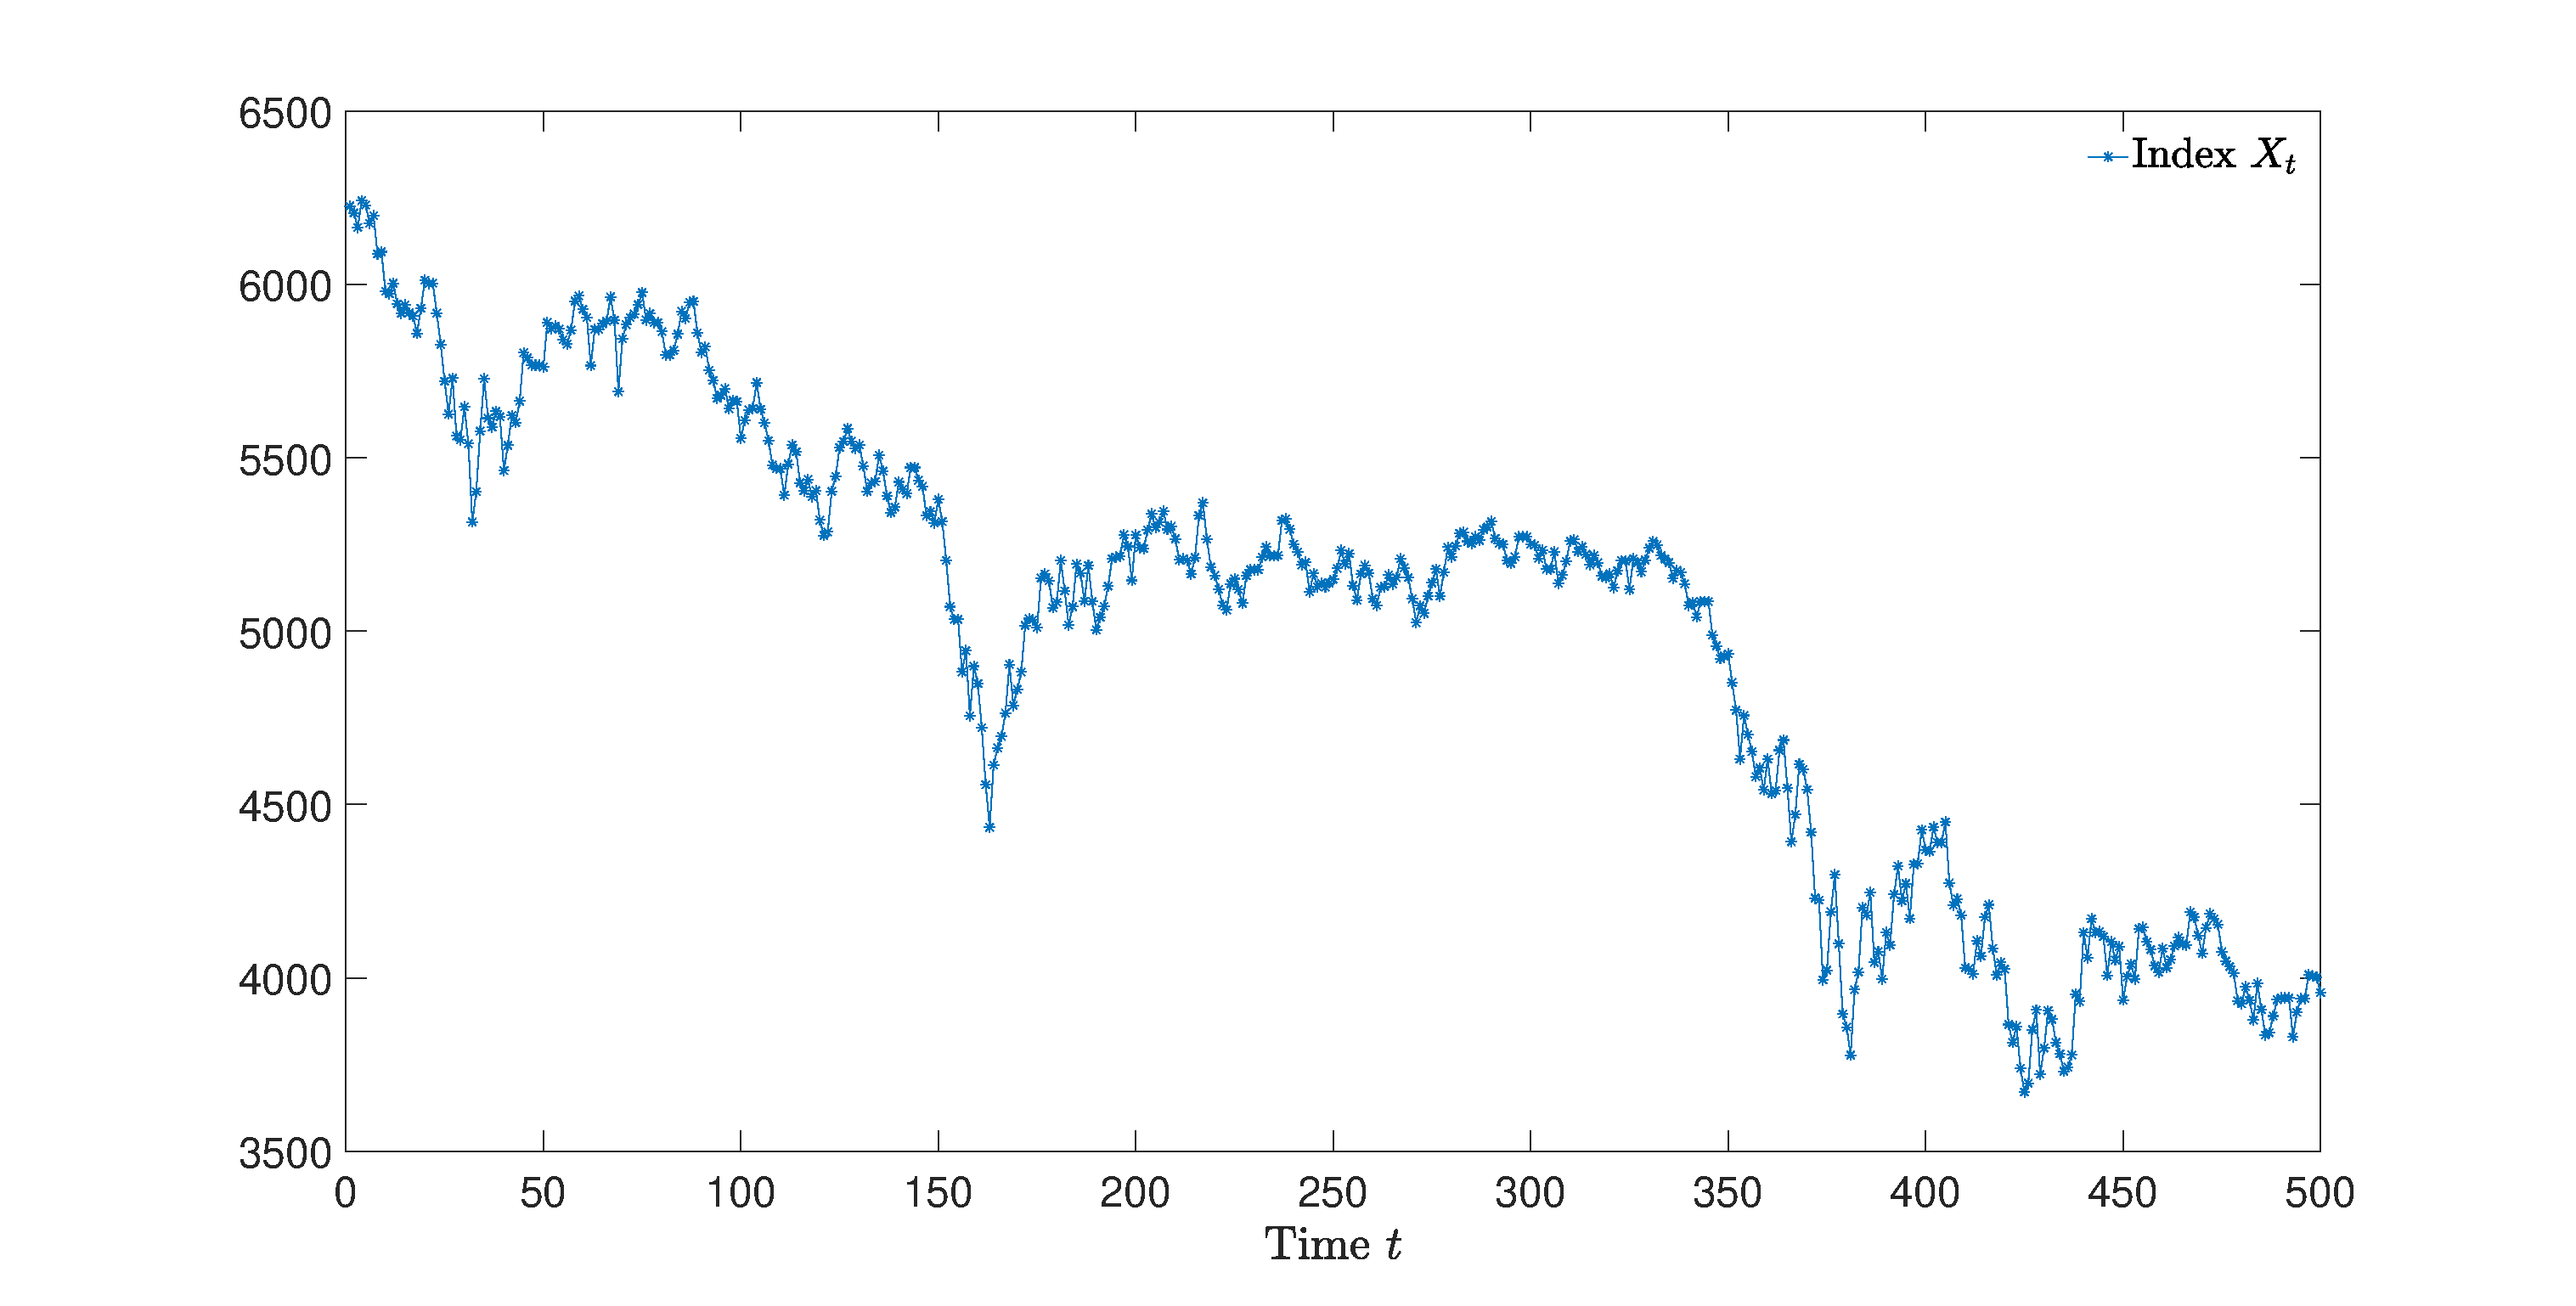
\includegraphics[width=1\textwidth]{data.eps}\\
        \caption{Data with 500 observed values}\label{data}
        \end{figure}

        Following the arguments above, try to fit the data through (\ref{OU}) by 

        i) choosing $\sigma=0$;

        ii) choosing $\sigma\neq0$;
    \end{question}
    We can rewrite the iteration expression as
    \[\hat X_{t+1}=
    \beta_0+\beta_1\hat X_t
    +\varepsilon_t\]
    where $\beta_0:=r\Delta t,\beta_1:=(1-\mu\Delta t)$
    and $\varepsilon_t:=\sigma(W_{t+\Delta t}-W_t)
    \sim\mathcal N(0,\sigma^2\Delta t)$.
    Then we can take advantage of statistic software to
    estimate the corresponded parameters as following.

    We denote the OLS estimates of $\beta_0,\beta_1,\sigma^2\Delta t$
    by $\hat\beta_0,\hat\beta_1,s^2$, then we have that
    \[\left\{\begin{aligned}
        \hat\beta_0&=\hat r\Delta t\\
        \hat\beta_1&=1-\hat\mu\Delta t\\
        s^2&=\hat\sigma^2\Delta t
    \end{aligned}\right.\]
    which is equivalent to
    \[\left\{\begin{aligned}
        \hat r&=\frac{\hat\beta_0}{\Delta t}\\
        \hat\mu&=\frac{1-\hat\beta_1}{\Delta t}\\
        \hat\sigma&=\sqrt{\frac{s^2}{\Delta t}}
    \end{aligned}\right.\]
    where $\hat r,\hat\mu,\hat\sigma$ are the estimates of $r,\mu,\sigma$
    accordingly.
    And we obtain the estimates as
    $\hat r=29.6,\hat\mu=0.00682,\hat\sigma=71.4$.

    When we choose $\sigma=0$, there is no stochastic pattern
    as $X_0=x_0$ is degenerated;
    when $\sigma\neq 0$, we can simulate a path.
    See \cref{fig:p5} for details.
    \begin{figure}[h]
        \centering
        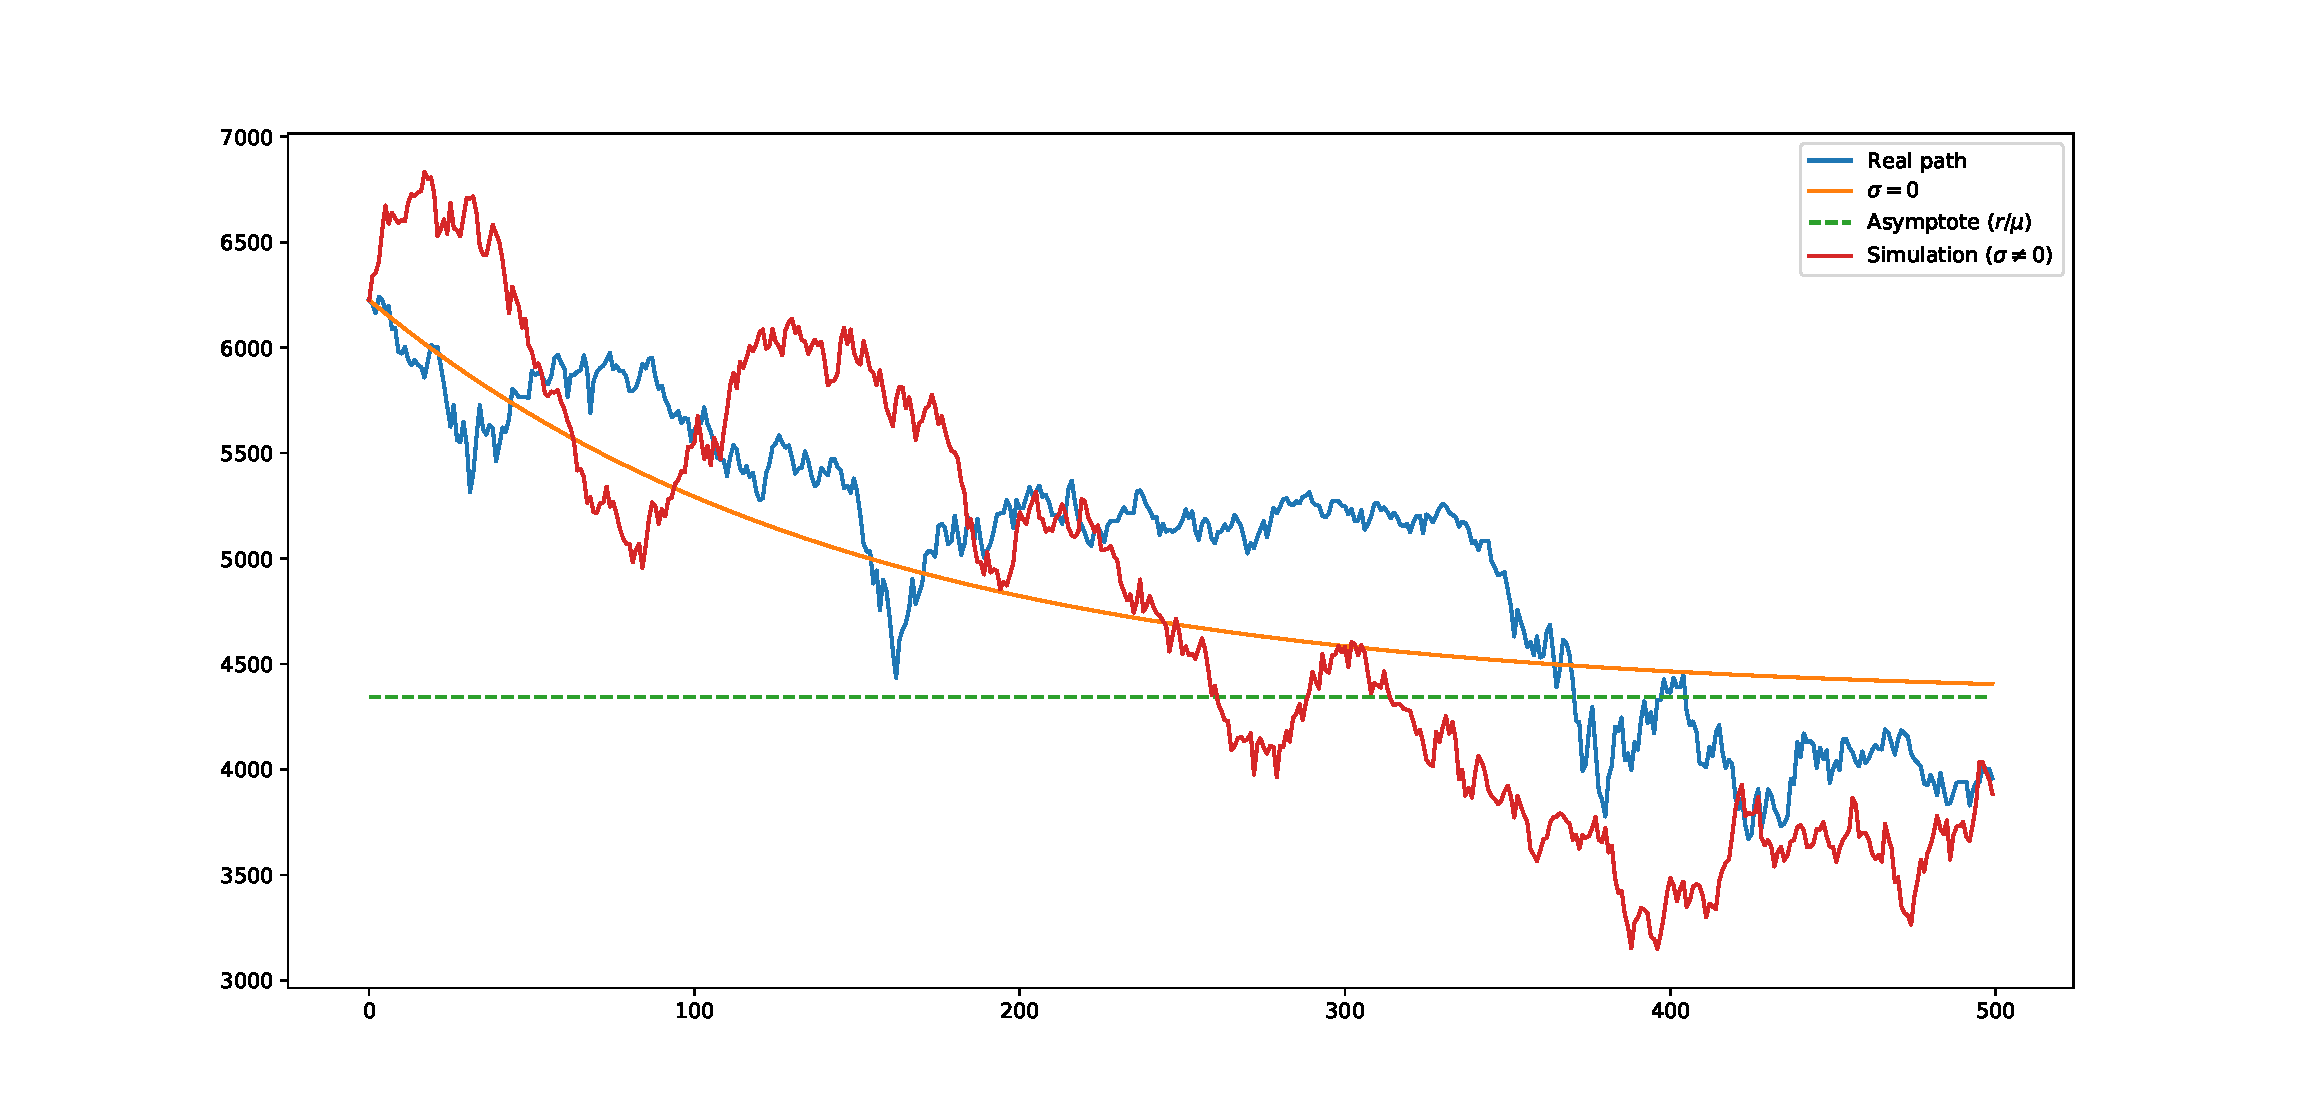
\includegraphics[width=\textwidth]{figure}
        \caption{Comparsion}
        \label{fig:p5}
    \end{figure}

    \newpage
    \appendix
    \section{Python Code for Graphing}
    \lstinputlisting[language=Python]{estimate.py}